%------------------------------------------------------------------------------
% Author(s):
% Varaun Ramgoolie
% Copyright:
%  Copyright (C) 2020 Brad Bachu, Arjun Mohammed, Nicholas Sammy, Kerry Singh
%
%  This file is part of Applied-Mathematics-Unit2 and is distributed under the
%  terms of the MIT License. See the LICENSE file for details.
%
%  Description:
%     Year: 2015
%     Module: 1
%     Question: 1
%------------------------------------------------------------------------------

\usetikzlibrary{patterns}

\begin{subquestions}

%------------------------------------------------------------------------------
% 1 a--------------------------------------------------------------------------
%------------------------------------------------------------------------------

\subquestion

Let $x$ be the number of cases of glass bottles and let $y$ be the number of cases of plastic bottles.

\begin{subsubquestions}

\subsubquestion

\begin{subsubsubquestions}

%------------------------------------------------------------------------------
% 1 a i a----------------------------------------------------------------------
%------------------------------------------------------------------------------

\subsubsubquestion

The profit function to be maximized is,

\begin{equation}
	P = 20x + 15y \,.
\end{equation}

%------------------------------------------------------------------------------
% 1 a i b----------------------------------------------------------------------
%------------------------------------------------------------------------------

\subsubsubquestion

The inequalities in this problem are,

\begin{align}
	x & \geq 0 \,, \nn \\
	y & \geq 0 \,, \nn \\
	4x + 4y & \leq 3000 \,, \nn \\
	3x + 6y & \leq 3000 \,.
\end{align}

\end{subsubsubquestions}

%------------------------------------------------------------------------------
% 1 a ii-----------------------------------------------------------------------
%------------------------------------------------------------------------------

\subsubquestion

\begin{subsubsubquestions}

%------------------------------------------------------------------------------
% 1 a ii a---------------------------------------------------------------------
%------------------------------------------------------------------------------
	
\subsubsubquestion

See Graph ~\ref{2015:q1:graph:Graph1}.

\begin{figure}
	\centering
	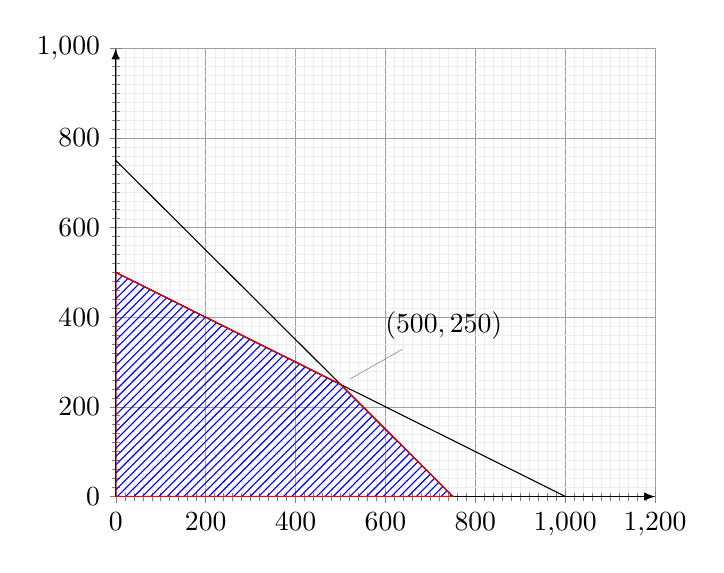
\begin{tikzpicture}
		\begin{axis}
			[
			xmin=-0,xmax=1200,
			ymin=0,ymax=1000,
			grid=both,
			grid style={line width=.1pt, draw=darkgray!10},
			major grid style={line width=.2pt,draw=darkgray!50},
			axis lines=left,
			minor tick num=9,
			enlargelimits={abs=0.5},
			axis line style={-latex},
			samples=100,
			domain = -20:20,
			]
	
			\addplot [mark=dot] coordinates{(1000,0)  (0,500)};
		
			\addplot [mark=dot] coordinates {(0,750) (750,0)};
		
			\addplot [mark=dot] coordinates {(0,500) (500,250) (750,0)};
			
			\addplot [red,pattern=north east lines,pattern color=blue] coordinates {(0,500) (500,250) (750,0)} \closedcycle;	

			\node [pin=45:{$(500,250)$}] at (axis cs:500,250) {};
			
		\end{axis}
	\end{tikzpicture}
	\caption{\label{2015:q1:graph:Graph1} Graph showing the feasible region of the problem.} 
\end{figure}

%------------------------------------------------------------------------------
% 1 a ii b---------------------------------------------------------------------
%------------------------------------------------------------------------------

\subsubsubquestion

The feasible region is shaded in Graph ~\ref{2015:q1:graph:Graph1}.

\end{subsubsubquestions}

%------------------------------------------------------------------------------
% 1 a iii ---------------------------------------------------------------------
%------------------------------------------------------------------------------

\subsubquestion

\begin{subsubsubquestions}
	
%------------------------------------------------------------------------------
% 1 a iii a -------------------------------------------------------------------
%------------------------------------------------------------------------------

\subsubsubquestion

Using \rdef{mod1:defn:TourOfvertices},

\begin{align}
	\text{Using (0,500)}\,, \nn \\
	P & = 20x + 15y\,, \nn \\
	  & = (20 \times 0) + (15 \times 500)\,, \nn \\
	  & = 7500\,. \\
	\text{Using (750,0)}\,, \nn \\
	P & = 20x + 15y\,, \nn \\
	  & = (20 \times 750) + (15 \times 0)\,, \nn \\
	  & = 15000\,. \label{2015:q1:eqn:Profit} \\	  
	\text{Using (500,250)}\,, \nn \\
	P & = 20x + 15y\,, \nn \\
	  & = (20 \times 500) + (15 \times250)\,, \nn \\
	  & = 13750\,.
\end{align}

To maximize the profit, $750$ cases of glass bottles and $0$ cases of plastic bottles should be manufactured.

%------------------------------------------------------------------------------
% 1 a iii b -------------------------------------------------------------------
%------------------------------------------------------------------------------

\subsubsubquestion

From \req{2015:q1:eqn:Profit}, the maximum profit is $\$ 15000$.

\end{subsubsubquestions}

\end{subsubquestions}

%------------------------------------------------------------------------------
% 1 b recheck this question ---------------------------------------------------
%------------------------------------------------------------------------------

\subquestion

The shortest path from Town S to Town G is,

\begin{equation}
	S \rightarrow C \rightarrow D \rightarrow F \rightarrow G ~\text{(20)} \,.
\end{equation}

The longest path from Town S to Town G is ,

\begin{equation}
	S \rightarrow D \rightarrow F \rightarrow E \rightarrow G ~\text{(31)} \,.
\end{equation}

\end{subquestions}

